\documentclass[aspectratio=169]{beamer}
\usetheme{Madrid}
\usecolortheme{dolphin}

\usepackage[T1]{fontenc}
\usepackage[utf8]{inputenc}
\usepackage{lmodern}
\usepackage{amsmath,amssymb}
\usepackage{booktabs}
\usepackage{graphicx}
\usepackage{hyperref}

\title[WTO/PNTR and U.S. Imports]{WTO Accession, PNTR, and U.S. Import Quantities and Prices}
\subtitle{}
\author{Vincent Zheng, Felix Yu, Aryan Goel}
\institute{University of Chicago}
\date{March 3, 2026}

\begin{document}

\begin{frame}
  \titlepage
\end{frame}

\begin{frame}{Talk Roadmap (12 min)}
  \small
  \begin{itemize}
    \item Research question and policy context
    \item Data and empirical strategy
    \item Main results and event-study evidence
    \item Limitations, robustness, and next steps
  \end{itemize}
\end{frame}

\begin{frame}{Background}

\end{frame}


\begin{frame}{Research Question}
  \begin{block}{Thesis question}
    How did the resolution of U.S. trade-policy uncertainty around China (PNTR in 2000, WTO accession in 2001/2002 implementation) affect:

    % make this less jargony
    \begin{itemize}
      \item import quantities into the U.S., and
      \item import prices paid by U.S. buyers?
    \end{itemize}
  \end{block}

\end{frame}


% \begin{frame}{Assumptions, Risks, and Robustness Plan}
%   \small
%   \textbf{Key assumptions}
%   \begin{itemize}
%     \item Parallel trends between more/less exposed products.
%     \item No confounding shocks perfectly aligned with exposure and timing.
%   \end{itemize}

%   \textbf{Current risks}
%   \begin{itemize}
%     \item Strong pre-trend rejections in some continuous event-study outcomes.
%     \item Potential measurement noise in unit values and quantity units.
%   \end{itemize}

%   \textbf{Planned robustness checks}
%   \begin{itemize}
%     \item Alternative post definitions and narrower windows.
%     \item Add controls for seasonality and unit-consistency filters.
%     \item Heterogeneity by Rauch classification and sector exclusions.
%   \end{itemize}
% \end{frame}
% add assumptions to the above slide


\begin{frame}{Policy Timing and Identification Intuition}
  \small
  \begin{itemize}
    \item Pre-2001: China receives renewable NTR treatment; ther is a risk for not receiving NTR, causing uncertainty to be priced into products.
    \item 2000: U.S. grants PNTR (legal permanence conditional on WTO accession).
    \item Dec 2001 / Jan 2002: WTO accession and operational transition.
  \end{itemize}

  \vspace{0.2cm}
  \begin{block}{Identification idea}
    Products with larger pre-period NTR gaps should respond more after policy uncertainty is resolved.
  \end{block}

  \begin{equation*}
    \text{Exposure}_p = \text{gap\_pre}_p = (\text{non-NTR tariff})_p - (\text{NTR tariff})_p
  \end{equation*}
\end{frame}

\begin{frame}{Identification idea}
  % describe DiD and how it evolves to the exposure (our treatment)
\end{frame}

\begin{frame}{Data and Sample}
  \small
  \textbf{Data sources}
  \begin{itemize}
    \item USITC monthly imports by product and HTS.
    \item Tariff schedule information used to construct product-level \texttt{gap\_pre}.
  \end{itemize}

  \textbf{Panel and outcomes}
  \begin{itemize}
    \item Product-month panel .
    \item Outcomes: \texttt{ln\_customs\_value}, \texttt{ln\_first\_unit\_qty}, \texttt{ln\_unit\_value}.
  \end{itemize}
\end{frame}

\begin{frame}{Baseline Specification}
  \small
  \begin{block}{Two-way FE DiD}
    \begin{equation*}
      Y_{pt} = \beta\,(\text{HighGap}_p \times \text{Post}_t) + \delta_p + \lambda_t + \varepsilon_{pt}
    \end{equation*}
  \end{block}

  \begin{itemize}
    \item $Y_{pt}$: log import value, log quantity, or log unit value.
    \item $\delta_p$: product fixed effects.
    \item $\lambda_t$: time fixed effects.
    \item SEs clustered at product level.
  \end{itemize}

  % \vspace{0.2cm}
  % \textbf{Continuous variant}
  % \begin{equation*}
  %   Y_{pt} = \theta\,(\text{gap\_pre}_p \times \text{Post}_t) + \delta_p + \lambda_t + \varepsilon_{pt}
  % \end{equation*}
  % add after if we have time 
\end{frame}

\begin{frame}{Main DiD Results (Current Outputs)}
  \small
  \textbf{Binary treatment (\texttt{HighGap x Post}) with product and date FE}
  \begin{itemize}
    \item \texttt{ln\_customs\_value}: $\hat\beta \approx 0.121$ (s.e. 0.031), positive and significant.
    \item \texttt{ln\_first\it\_qty}: $\hat\beta \approx 0.145$ (s.e. 0.036), positive and significant.
    \item \texttt{ln\_unit\_value}: $\hat\beta \approx -0.024$ (s.e. 0.017), negative but not strongly significant in FE spec.% explain why this might be (noisy proxy for price)
          % explain why these numbers make sense intuitively

  \end{itemize}
  % check numbers

  \vspace{0.2cm}
  \textbf{Interpretation}
  \begin{itemize}
    \item High-gap products show stronger post-policy growth in value and quantity.
    \item Price effects are weaker in the binary split and clearer in continuous treatment.
  \end{itemize}
\end{frame}


% \begin{frame}{Continuous-Treatment Results}
%   \small
%   From \texttt{did\_continuous\_gap\_pre\_post\_effects.csv}:
%   \begin{itemize}
%     \item Value (\texttt{ln\_customs\_value}): $\hat\theta = 0.122$ (s.e. 0.134).
%     \item Quantity (\texttt{ln\_first\_unit\_qty}): $\hat\theta = -0.061$ (s.e. 0.130).
%     \item Unit value (\texttt{ln\_unit\_value}): $\hat\theta = -0.131$ (s.e. 0.032), strong negative effect.
%   \end{itemize}

%   \vspace{0.2cm}
%   \begin{block}{Reading}
%     Higher tariff-jump exposure is associated with stronger post-policy price declines, consistent with lower import prices in more exposed products.
%   \end{block}
% \end{frame}

\begin{frame}{Event Study: Value and Quantity}
  \centering
  \begin{columns}[T,onlytextwidth]
    \begin{column}{0.49\textwidth}
      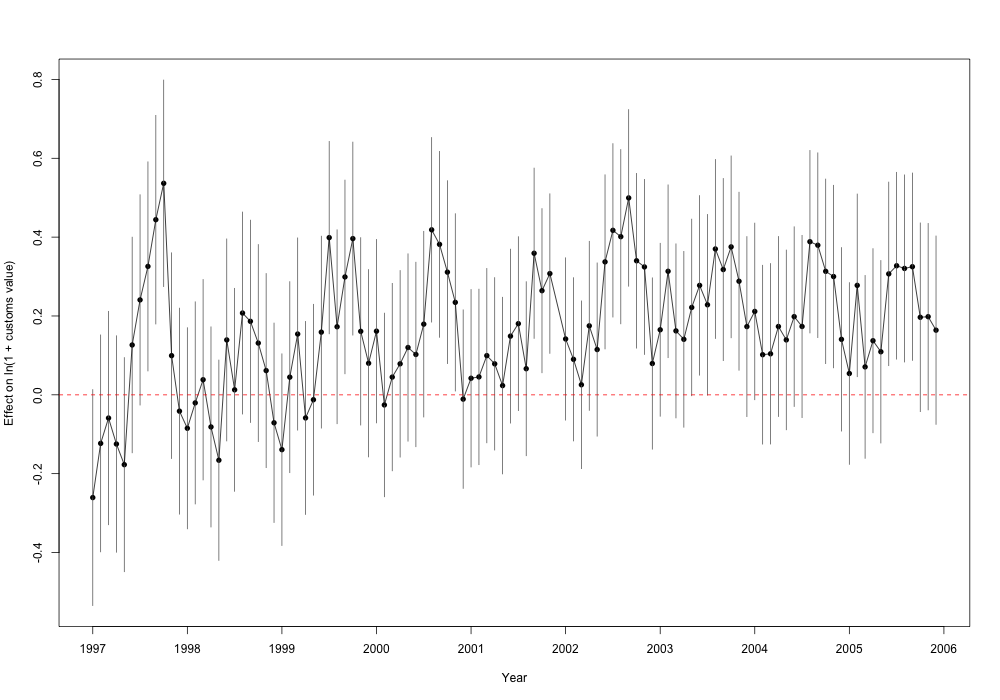
\includegraphics[width=\linewidth]{../analysis/results/figures/event_study/event_study_ln_customs_value.png}
      \vspace{0.1cm}
      \scriptsize Value event study
    \end{column}
    \begin{column}{0.49\textwidth}
      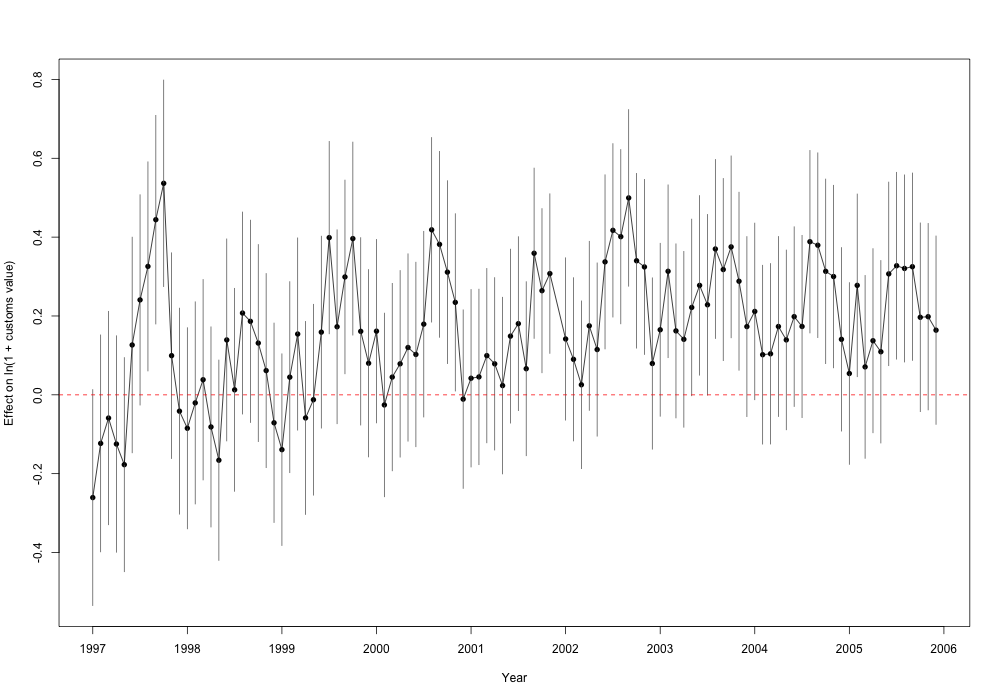
\includegraphics[width=\linewidth]{../analysis/results/figures/event_study/event_study_ln_first_unit_qty.png}
      \vspace{0.1cm}
      \scriptsize Quantity event study
    \end{column}
  \end{columns}
\end{frame}

% add notes to talk during presentation (intuition wise) 

\begin{frame}{Event Study: Unit Value (Price Proxy)}
  \centering
  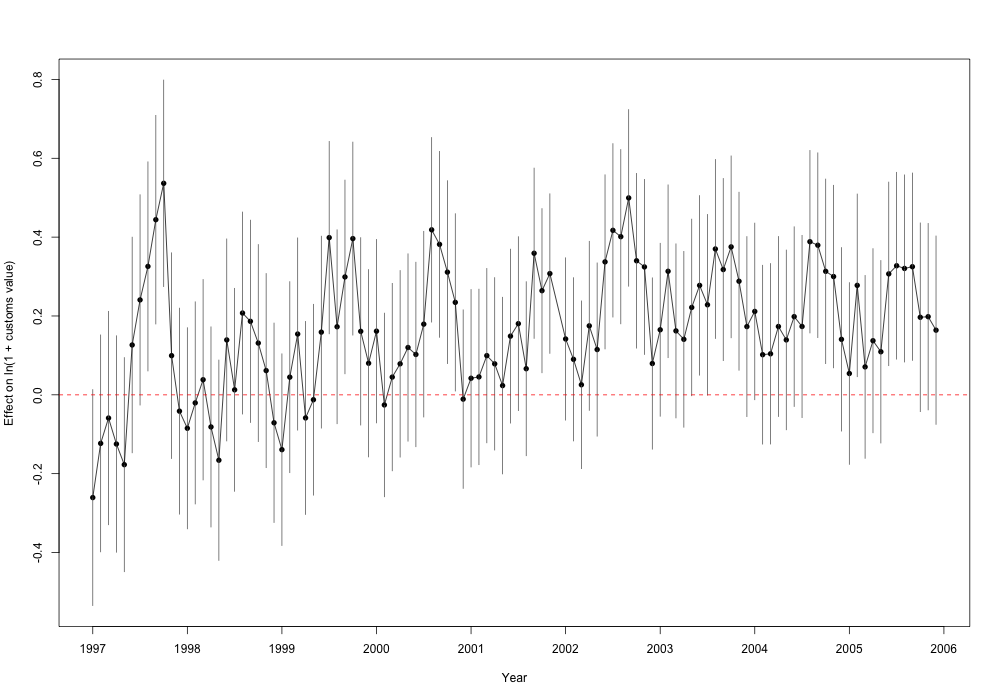
\includegraphics[height=0.62\textheight,keepaspectratio]{../analysis/results/figures/event_study/event_study_ln_unit_value.png}

  \vspace{0.2cm}
  \scriptsize
  Continuous-treatment pre-trend test for unit value: $p \approx 0.081$ (marginal).
\end{frame}

\begin{frame}{Takeaways and Next Steps}
  \small
  \textbf{Takeaways}
  \begin{itemize}
    \item Evidence supports a post-policy increase in import value and quantity for high-gap products.  \end{itemize}

  \textbf{Next steps}
  \begin{itemize}
    \item empty
          % written by Vincent
  \end{itemize}
\end{frame}

\begin{frame}
  \centering
  \Large Questions
\end{frame}

\end{document}
